\documentclass[aspectratio=169]{beamer}

\usetheme{Boadilla}
\usecolortheme{default}

\usepackage[T1]{fontenc}
\usepackage[utf8]{inputenc}
\usepackage{booktabs}
\usepackage{listings}
\usepackage{tikz}
\usetikzlibrary{arrows.meta,positioning,calc}

\definecolor{GLBlue}{RGB}{22,63,95}
\definecolor{GLGray}{RGB}{96,104,114}
\definecolor{GLLight}{RGB}{232,240,248}

\setbeamercolor{normal text}{fg=black,bg=white}
\setbeamercolor{title}{fg=GLBlue}
\setbeamercolor{subtitle}{fg=GLGray}
\setbeamercolor{frametitle}{fg=GLBlue,bg=GLBlue!6}
\setbeamercolor{titlelike}{fg=GLBlue}
\setbeamercolor{author}{fg=GLGray}
\setbeamercolor{date}{fg=GLGray}
\setbeamercolor{structure}{fg=GLBlue}
\setbeamercolor{itemize item}{fg=GLBlue}
\setbeamercolor{itemize subitem}{fg=GLGray}

\setbeamerfont{title}{size=\LARGE,series=\bfseries}
\setbeamerfont{subtitle}{size=\normalsize}
\setbeamerfont{frametitle}{size=\Large,series=\bfseries}

\setbeamertemplate{navigation symbols}{}
\setbeamertemplate{headline}{}
\setbeamertemplate{footline}[frame number]
\setbeamertemplate{itemize subitem}[triangle]

\lstset{
  language=Python,
  basicstyle=\ttfamily\footnotesize,
  keywordstyle=\color{GLBlue}\bfseries,
  commentstyle=\color{GLGray}\itshape,
  stringstyle=\color{GLBlue!70!black},
  backgroundcolor=\color{GLLight},
  frame=single,
  rulecolor=\color{GLBlue},
  columns=fullflexible,
  keepspaces=true,
  showstringspaces=false,
  xleftmargin=4pt,
  xrightmargin=4pt,
}

\title{Column generation in rcspp}
\subtitle{Where it stands, what works, what is next}
\author{Leo Marbehan}
\date{November 2, 2026}

\begin{document}

\begin{frame}[plain]
  \titlepage
\end{frame}

%--------------------------------------------------------------
\begin{frame}{Presentation Outline}
  \begin{enumerate}
    \item Goal and design
    \item Work completed
    \item Measurements: correctness and timing
    \item Lessons, limits and next steps
    \item Discussion
  \end{enumerate}
\end{frame}

%--------------------------------------------------------------
\begin{frame}{Goal and design}
  \framesubtitle{Goal}

  \begin{itemize}
    \item \textbf{Ship column generation ready to use} on top of the RCSPP solver
      \begin{itemize}
        \item Small: rcspp is about the pricer, the layer only drives it
        \item Customizable in C++ and in Python: master solver, pricing stages, initialization
        \item Not changing how rcspp works today
      \end{itemize}
    \item \textbf{Its own library and build option}
      \begin{itemize}
        \item The core builds and passes its 597 tests without it
        \item Opt-in: \texttt{rcspp.hpp} does not include it, it has its own headers
        \item Python: one wheel (about 3.4 MB) with HiGHS inside, no extra import time
      \end{itemize}
  \end{itemize}
\end{frame}

%--------------------------------------------------------------
\begin{frame}{Goal and design}
  \framesubtitle{Architecture}

  \vspace{0.6em}
  \begin{center}
  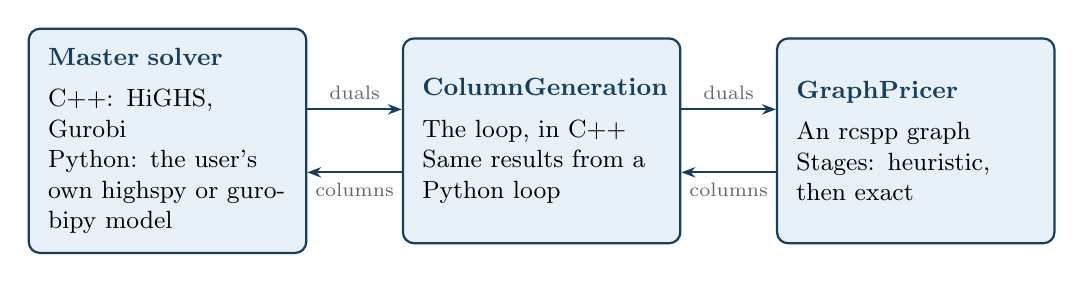
\begin{tikzpicture}[
      box/.style={
        draw=GLBlue, thick, rounded corners=4pt,
        fill=GLLight, text width=0.25\textwidth,
        minimum height=2.6cm, align=left, inner sep=7pt,
        font=\small
      },
      arr/.style={-{Stealth[length=5pt]}, GLBlue, thick}
    ]
    \node[box] (master) {%
      {\color{GLBlue}\textbf{Master solver}}\\[4pt]
      C++: HiGHS, Gurobi\\
      Python: the user's own highspy or gurobipy model};
    \node[box, right=1.2cm of master] (loop) {%
      {\color{GLBlue}\textbf{ColumnGeneration}}\\[4pt]
      The loop, in C++\\
      Same results from a Python loop};
    \node[box, right=1.2cm of loop] (pricer) {%
      {\color{GLBlue}\textbf{GraphPricer}}\\[4pt]
      An rcspp graph\\
      Stages: heuristic, then exact};
    \draw[arr] ([yshift=4mm]master.east) -- node[above, font=\scriptsize, GLGray] {duals} ([yshift=4mm]loop.west);
    \draw[arr] ([yshift=-4mm]loop.west) -- node[below, font=\scriptsize, GLGray] {columns} ([yshift=-4mm]master.east);
    \draw[arr] ([yshift=4mm]loop.east) -- node[above, font=\scriptsize, GLGray] {duals} ([yshift=4mm]pricer.west);
    \draw[arr] ([yshift=-4mm]pricer.west) -- node[below, font=\scriptsize, GLGray] {columns} ([yshift=-4mm]loop.east);
  \end{tikzpicture}
  \end{center}

  \vspace{0.6em}
  \begin{itemize}
    \item Each box is an interface: a user can replace any of them
    \item The pricer reuses the existing algorithms; nothing changed in the graph code
  \end{itemize}
\end{frame}

%--------------------------------------------------------------
\begin{frame}{Goal and design}
  \framesubtitle{Critical decisions}

  \footnotesize
  \begin{tabular}{p{0.19\textwidth}p{0.35\textwidth}p{0.38\textwidth}}
    \toprule
    \textbf{Question} & \textbf{Decision} & \textbf{Why} \\
    \midrule
    Where does the code live? & In C++, bound to Python; a Python loop as an example, built on the C++ pieces
      & One implementation; pricing, the costly part, stays in C++ \\
    \addlinespace
    \textit{Open:} more in Python? & Possibly duplicate a few pieces in Python
      & More freedom for Python-only users \\
    \addlinespace
    Master from Python? & Wrap the user's own highspy or gurobipy model & Users already write their master; no duplication \\
    \addlinespace
    Which LP solver? & HiGHS by default (in the wheel), Gurobi optional
      & Runs and is tested without a license; HiGHS about 8$\times$ faster than SoPlex on public LP benchmarks \\
    \addlinespace
    SCIP? & Not for column generation alone & Adds overhead over a direct LP solver; an option later for branch-and-price \\
    \addlinespace
    Gurobi from Python? & Through gurobipy for now & Next slide \\
    \bottomrule
  \end{tabular}
\end{frame}

%--------------------------------------------------------------
\begin{frame}{Goal and design}
  \framesubtitle{Gurobi from Python}

  \textbf{The problem}: our Gurobi master solver uses Gurobi's C++ API, compiled per compiler.
  A pip wheel cannot ship it, and gurobipy only ships Gurobi's C library.

  \vspace{0.5em}
  \footnotesize
  \begin{tabular}{p{0.06\textwidth}p{0.3\textwidth}p{0.17\textwidth}p{0.35\textwidth}}
    \toprule
    \textbf{Route} & \textbf{How} & \textbf{Who can use it} & \textbf{Cost} \\
    \midrule
    A & A Python master solver over gurobipy \textbf{(available)}
      & Anyone with gurobipy & Python in each iteration \\
    \addlinespace
    B1 & Copy the gurobipy model into the C++ master solver
      & Source builds with Gurobi & Two copies of Gurobi's library in one process, same version required \\
    \addlinespace
    B2 & A master solver on Gurobi's C API, using the library gurobipy already loaded
      & Anyone with gurobipy, from the wheel & A rewrite on the C API, adapters per Gurobi version \\
    \bottomrule
  \end{tabular}

  \vspace{0.5em}
  \small
  \begin{itemize}
    \item Cost of A, measured: adding a column 13--25\,$\mu$s against 4--10\,$\mu$s in C++;
      1 to 15\% per iteration on small, fast LPs
    \item On the VRP instances: not measurable, pricing dominates
    \item Next: build B1 and B2 far enough to test, time A, B1 and B2, then decide
  \end{itemize}
\end{frame}

%--------------------------------------------------------------
\begin{frame}[fragile]{Goal and design}
  \framesubtitle{How a user writes it (Python)}

\begin{lstlisting}
import rcspp.column_generation as cg

graph = build_graph(instance)  # an rcspp graph; each arc lists the master rows it covers
master = cg.MasterProblem(cg.HighsMasterSolver(row_lower=lower, row_upper=upper))
# or: cg.HighspyMasterSolver(my_highs_model), cg.GurobipyMasterSolver(my_gurobi_model)

master.add_pricer(cg.GraphPricer(graph, [cg.PricingStage("simple")]), cg.ConvexityRow())
result = cg.ColumnGeneration(master, cg.ColumnGenerationParams()).run()

print(result.status, result.objective, result.iterations)
\end{lstlisting}

  \begin{itemize}
    \item C++ has the same shape: \texttt{MasterProblem}, \texttt{add\_pricer}, \texttt{ColumnGeneration::run}
    \item The master takes several pricers (for example one per vehicle type): one \texttt{add\_pricer} call each
  \end{itemize}
\end{frame}

%--------------------------------------------------------------
\begin{frame}{Work completed}
  \framesubtitle{Status}

  \begin{itemize}
    \item \textbf{C++ layer}: done, four stacked draft PRs
      \begin{itemize}
        \item Interfaces, master problem and loop; Gurobi master solver; graph pricer; HiGHS master solver
        \item A shared self-test for every master solver (dual signs, warm start, added columns)
      \end{itemize}
    \item \textbf{Python layer}: done in code
      \begin{itemize}
        \item Bindings, the highspy and gurobipy master solvers, a Python loop as an example
      \end{itemize}
    \item \textbf{Packaging}: done, draft PR
      \begin{itemize}
        \item Build options, CMake components and install rules
      \end{itemize}
    \item \textbf{Measurements}: done, against both current VRP examples
  \end{itemize}
\end{frame}

%--------------------------------------------------------------
\begin{frame}{Measurements}
  \framesubtitle{Setup}

  \begin{itemize}
    \item \textbf{Solomon VRPTW instances}, 12 to 100 customers, cycles allowed (no ng-routes)
    \item \textbf{Compared}:
      \begin{itemize}
        \item The current Python example (python-mip with Gurobi) and C++ example (Gurobi)
        \item The new layer: C++ loop or Python loop $\times$ HiGHS (C++), highspy, gurobipy
      \end{itemize}
    \item \textbf{Same relaxation} for all; the layer prices on the Python example's graph, exact pricing
  \end{itemize}

  \vspace{0.4em}
  \textbf{Caveat: quick measurements, done for this meeting}
  \begin{itemize}
    \item The goal was a first insight into results and performance, not a benchmark
    \item One run each, on my non-idle desktop (other processes used 0.5 to 1 core)
    \item Timings are indicative; differences under about 20\% are noise
  \end{itemize}
\end{frame}

%--------------------------------------------------------------
\begin{frame}{Measurements}
  \framesubtitle{Correct, and on a par with the examples}

  \small
  \textbf{LP values: identical in every run that finished, on all 13 instances, and equal to the recorded
  baseline where one exists}

  \vspace{0.6em}
  \centering
  \begin{tabular}{lrrrrr}
    \toprule
    \textbf{Solve time (s)} & \textbf{C101} & \textbf{R101} & \textbf{RC101} & \textbf{C201} & \textbf{R201} \\
    \midrule
    Python example & 2.5 & 1.0 & 1.5 & 51 & 1745 \\
    C++ example & 3.1 & 0.8 & 1.5 & 53 & 2093 \\
    Layer, 6 configurations & 1.6--2.5 & 0.5--0.6 & 1.0--1.1 & 25--37 & 1730--1980 \\
    \bottomrule
  \end{tabular}

  \vspace{0.8em}
  \begin{itemize}
    \item Layer started from single-customer routes, as the examples start
    \item \textbf{C++ loop or Python loop: no measurable difference} (Python overhead under 0.1 s)
    \item C201 looks faster with the layer, but it comes from fewer iterations
      (different duals), not from faster code: \textbf{no speed claim}
  \end{itemize}
\end{frame}

%--------------------------------------------------------------
\begin{frame}{Measurements}
  \framesubtitle{Where the time goes}

  \small
  \centering
  \begin{tabular}{lrrr}
    \toprule
    \textbf{Master time per iteration (s)} & \textbf{C201} & \textbf{RC201} & \textbf{R201} \\
    \midrule
    HiGHS & 0.14 & 0.42 & 0.88 \\
    Gurobi (gurobipy) & 0.05 & 0.06 & 0.12 \\
    \midrule
    Master share of the solve time & 48--73\% & 0.3--2\% & 0.3--2\% \\
    \bottomrule
  \end{tabular}

  \vspace{0.8em}
  \begin{itemize}
    \item \textbf{R2 and RC2: pricing is over 95\% of the time}, the master solver does not matter
    \item \textbf{C2: the master dominates}, and Gurobi solves each LP 3 to 7 times faster than HiGHS
    \item HiGHS from C++ or through highspy: same time
  \end{itemize}
\end{frame}

%--------------------------------------------------------------
\begin{frame}{Lessons}
  \framesubtitle{The default start}

  \textbf{Starting without columns}: one artificial column per row, with a large cost
  \begin{itemize}
    \item The automatic cost is $10^6 \times$ the largest arc cost: about $7 \cdot 10^7$ on R2 instances
    \item HiGHS stops with ``excessive dual values''
      \begin{itemize}
        \item At once on R201\_25 and RC201\_12, after about an hour on R201
      \end{itemize}
    \item Gurobi finishes R201, but in about 7000 s instead of 1745 s
    \item On R201, the first pricing alone took about an hour (52 to 59 min):
      longer than a whole run from single-customer routes (about 30 min)
  \end{itemize}

  \vspace{0.4em}
  \textbf{Workarounds that already work}
  \begin{itemize}
    \item Start from single-customer routes (as the examples do): all configurations solve, on a par
    \item A smaller explicit cost ($10^5$) also fixed R201\_25
  \end{itemize}

  \vspace{0.4em}
  \textbf{To understand first}, then fix before shipping (a safer automatic cost, or a fallback in HiGHS?)
\end{frame}

%--------------------------------------------------------------
\begin{frame}{Lessons}
  \framesubtitle{Heuristic pricing and limits}

  \textbf{Heuristic stage (greedy, then exact)}
  \begin{itemize}
    \item Without a cap on the number of columns, greedy returned about 140{,}000 columns per call on C101\_25
    \item 5 to 16 s instead of 1 s, and memory filled up on R201\_25
    \item The cap exists (\texttt{stop\_after\_X\_solutions}); open question: a default cap, or only documentation?
    \item Quick check with a cap of 100 (laptop): about 2{,}800 columns, under 1 s;
      on these small instances still slower than exact pricing alone
  \end{itemize}

  \vspace{0.4em}
  \textbf{Limits of these measurements}
  \begin{itemize}
    \item Cycles allowed only: no ng-routes, no elementary routes; 100 customers at most
    \item One run per configuration on a busy machine
    \item Not competitive with state-of-the-art branch-price-and-cut solvers (ng-routes, bucket labeling, cuts):
      that is the pricing algorithm, not the layer
  \end{itemize}
\end{frame}

%--------------------------------------------------------------
\begin{frame}{Next steps}

  \begin{enumerate}
    \item \textbf{Dig deeper into the lessons and findings of the measurements} before changing anything
    \item \textbf{Gurobi from Python}: test routes B1 and B2, compare with A
    \item \textbf{Comparison with ng-routes} with the existing C++ comparison program
    \item \textbf{User documentation page}, then the PRs out of draft
    \item Later: stabilization, Lagrangian bound, column pool; branch-and-price is designed, not decided
  \end{enumerate}
\end{frame}

%--------------------------------------------------------------
\begin{frame}{Discussion}

  \begin{itemize}
    \item \textbf{What should the next steps be, in your view?}
    \item \textbf{What do you want the column generation feature to become?}
      \begin{itemize}
        \item Column generation only, or towards branch-and-price?
        \item Which users first: C++, Python, or both equally?
        \item What would ``ready to ship'' mean for you?
      \end{itemize}
  \end{itemize}
\end{frame}

%--------------------------------------------------------------
\begin{frame}{Backup}
  \framesubtitle{LP solvers: HiGHS, SoPlex and SCIP}

  \small
  \centering
  \begin{tabular}{lll}
    \toprule
    & \textbf{HiGHS 1.15} & \textbf{SoPlex 8.1} \\
    \midrule
    Mittelmann LP benchmark (1 = fastest) & \textbf{12.8}, 54/65 solved & 101, 34/65 solved \\
    Network LPs & \textbf{5.9} & 33.0 \\
    Exact (rational) LP & No & \textbf{Yes} \\
    Python package & \textbf{highspy on PyPI} & None on PyPI \\
    License & MIT & Apache-2.0 \\
    \bottomrule
  \end{tabular}

  \raggedright
  \vspace{0.6em}
  \begin{itemize}
    \item Benchmarks are cold solves of large LPs; nobody publishes re-solves after added columns, our case
    \item \textbf{SoPlex}: only for exact checks, or as SCIP's default LP solver
    \item \textbf{SCIP, column generation alone}: presolve and a transformed problem on top of the LP;
      SCIP's own FAQ advises calling an LP solver directly
    \item \textbf{SCIP, branch-and-price}: a serious option with rcspp as SCIP's pricer (tree, node warm starts,
      heuristics built in); costs a large API and a mostly sequential solver
  \end{itemize}
\end{frame}

\end{document}
